\documentclass[conference]{IEEEtran}
\IEEEoverridecommandlockouts
% The preceding line is only needed to identify funding in the first footnote. If that is unneeded, please comment it out.
\usepackage{cite}
\usepackage{algorithmic}
\usepackage{graphicx}
\usepackage{textcomp}
\usepackage{amsmath}
\usepackage[sc]{mathpazo}
\usepackage{datetime}
\usepackage{graphicx, wrapfig, subcaption, setspace, booktabs}
\usepackage[T1]{fontenc}
\usepackage{fourier}
\usepackage{url, lipsum}
\usepackage{hyperref,bookmark}
\usepackage[T1]{fontenc}
\usepackage{amssymb}
\usepackage{makecell, multirow, tabularx}
\usepackage{listings}
\usepackage[ruled,linesnumbered,vlined]{algorithm2e}

\usepackage{float}
\usepackage{nomencl}
\usepackage{ifthen}

\renewcommand{\nomgroup}[1]{%
	\ifthenelse{\equal{#1}{P}}{\item[\textbf{Parameters}]}{%
		\ifthenelse{\equal{#1}{V}}{\item[\textbf{Variables \\}]}}
}
\makenomenclature
\def\BibTeX{{\rm B\kern-.05em{\sc i\kern-.025em b}\kern-.08em
    T\kern-.1667em\lower.7ex\hbox{E}\kern-.125emX}}
\begin{document}

\title{CO\textsubscript{2} and Cost Impacts on a Transportation Microgrid with Electric Vehicle Charging Infrastructure: a case study in Southern California}

\author{
	\IEEEauthorblockN{Luis Fernando Enriquez-Contreras\IEEEauthorrefmark{1}\IEEEauthorrefmark{2}, Matthew Barth\IEEEauthorrefmark{1}\IEEEauthorrefmark{2}, Sadrul Ula\IEEEauthorrefmark{2}}
	\IEEEauthorblockA{\IEEEauthorrefmark{1}\textit{Department of Electrical  and Computer Engineering} \\
		\textit{University of California, Riverside}\\
				Riverside, United States of America \\
				lenri001@ucr.edu, barth@ece.ucr.edu}
	\IEEEauthorblockA{\IEEEauthorrefmark{2}\textit{College of Engineering, Center for Environmental Research \& Technology} \\
		\textit{University of California, Riverside}\\
				Riverside, United States of America \\
				lenri001@ucr.edu, barth@ece.ucr.edu, sula@cert.ucr.edu}
}
\maketitle

\begin{abstract}

	As an important part of Intelligent Transportation Systems (ITS), this paper presents a case study at the University of California, Riverside (UCR) that evaluates the effectiveness of different transportation-based microgrid configurations in reducing both carbon dioxide (CO\textsubscript{2}) emissions and electricity costs. The CO\textsubscript{2} emissions are calculated using high-resolution California Independent System Operator (CAISO) CO\textsubscript{2} emissions data to accurately assess the environmental impact of each setup. Electric costs were also compared to determine the financial savings potential for the consumer. The results demonstrate that a peak-shaving transportation-microgrid can effectively reduce CO\textsubscript{2} emissions in the range of 24\% to 38\% and costs from \$27,000 to \$29,000 per year, even when considering the additional demand from the 12 vehicles charging daily at the building. However, careful consideration should be given to battery sizing, as peak-shaving has diminishing returns. Doubling the battery size may only provide an additional savings of \$2,000 per year with a negligible reduction in emissions. This highlights the importance of optimizing battery capacity to maximize cost-effectiveness and environmental impact.
	

\end{abstract}

\begin{IEEEkeywords}
microgrids, demand response, CO\textsubscript{2} emissions, modelica, EV charging
\end{IEEEkeywords}


\section{Introduction}
    \subsection{Background}
		California is committed to reducing greenhouse gas emissions through various approaches. However, two large contributors to greenhouse gas emissions in California are transportation and electricity generation.  In California, electric vehicles (EVs) accounted for 25.4\% of Q2 2023 vehicle sales \cite{ev_sale_percentage}, and the state aims to ban the sale of internal combustion engine vehicles by 2035 \cite{ice_ban}. Concurrently, California is expanding the number of charging stations in the state, reaching over 13,844 Level 2 and 1,924 Level 3 stations \cite{ev_stations_CA} as of November . EV technology has advanced, and new EVs can charge up to 80\% in 20-60 minutes \cite{ev_stats}. This is enabled by Level 3 charging, which can deliver up to 350 kilowatts (kW), compared to Level 2 charging, which is limited to 19 kW \cite{ev_stats}. While this reduced charging time has increased the attractiveness of EVs, it also poses a challenge for the owners of these chargers, as they can generate a large amount of electricity demand quickly. As California strives to increase the share of clean energy in its electricity mix, it also needs to reduce the CO\textsubscript{2} emissions from transportation by promoting electrification. This leads to two conundrums: how will California provide enough capacity for electrified transportation, and how clean is the grid to minimize the emissions associated with battery electric vehicles? One method to alleviate the pressure on the grid is to localize electricity production and EV charging by using microgrids. A microgrid is defined by the Department of Energy (DOE) and the Institute of Electrical and Electronics Engineers (IEEE) as: “a group of interconnected loads and distributed energy resources within clearly defined electrical boundaries that acts as a single controllable entity with respect to the grid. A microgrid can connect and disconnect from the grid to enable it to operate in both grid-connected or island-mode.” \cite{microgrid_def} \cite{microgrid_def_ieee}. As microgrids and EV chargers become more widespread, it is essential to study the economic and environmental impacts of EV charging, especially fast charging, and how microgrids can play an important role. EV charging differs from typical building loads, as it can rapidly ramp up to high levels at random intervals based on human behavior i.e. when they plug in. An outlier event where multiple people charge at the same time can cause a significant peak in the load. \\
		
		This research holds significant implications for the advancement of intelligent transportation systems, as it aims to address the economic needs of EV charging infrastructure owners and determine the optimal configuration that benefits both EV owners and the environment by minimizing greenhouse gas emissions. This paper delves into the impacts of transportation microgrids equipped with Level 2 and Level 3 charging on the behavior of microgrids, associated electricity costs, and CO\textsubscript{2} emissions within the context of southern California. The simulations are conducted using OpenModelica, a dynamic modeling and simulation environment. This study distinguishes itself from previous research in many ways, including employing a higher time resolution for calculating CO\textsubscript{2} emissions, capturing data every 15 minutes.
		
%		This work is crucial for the field of intelligent transportation systems since new EVs should also be beneficial to those who own EV charging infrastructure. Understanding the economic needs of EV chargers owner, and what setup can be beneficial for them, EV owners, and best reduce greenhouse gas emissions from the environment ia s topic that needs to be further investigated. This paper analyzes the impacts of transportation microgrids with Level 2 and Level 3 charging on the behavior of microgrids and the associated electric costs and CO\textsubscript{2} emissions in southern California. The simulation is run in OpenModelica, which is a dynamic modeling and simulation environment. This paper also uses a higher time resolution data than most studies to calculate the CO\textsubscript{2} emissions every 15 minutes.
  	\subsection{Literature Review}
  		Transportation microgrids have gained significant traction in recent years due to the growing demand for transportation electrification. These microgrids, which combine distributed energy resources (DERs) and energy storage systems with electric vehicle (EV) charging infrastructure, offer a promising solution for integrating EVs into the power grid while minimizing environmental impact. Previous studies have investigated the economic viability of transportation microgrids, primarily focusing on energy charges associated with EV charging. However, demand charges, which reflect the peak demand imposed on the grid, need to be addressed. This omission is particularly crucial for fast charging stations, which draw significant power during peak periods. A more comprehensive approach to economic analysis should consider both energy and demand charges, providing a more accurate assessment of the overall cost of operating a transportation microgrid. Research has addressed the impact of EV charging demand on transportation microgrids, often focusing on low-demand Level 2 charging. However, the increasing popularity of high-demand Level 3 charging requires a more nuanced understanding of its implications. Studies should incorporate a mix of Level 2 and Level 3 charging scenarios to accurately assess the impact of EV charging demand on microgrid operation and economics. Assessing the greenhouse gas (GHG) emissions associated with transportation microgrids is often simplified by using average CO\textsubscript{2} emissions from an area's electricity production. This approach fails to capture the variations in CO\textsubscript{2} emissions throughout the day, which can significantly affect the environmental impact of EV charging. More sophisticated GHG emission calculations should consider the time-varying nature of CO\textsubscript{2} emissions, providing a more accurate representation of the environmental impact of transportation microgrids. \\
  		
  		Several studies have investigated the performance of electric vehicle charging stations (EVCS) under varying conditions. Reference \cite{himabindu2021analysis}, is developing a demand and stochastic model for EVCS, followed by a techno-economic assessment and an environmental impact analysis. They concluded that the optimal configuration and investment costs of EVCS with solar integration are highly dependent on feed-in tariffs and solar irradiation levels. However, their CO\textsubscript{2} emission calculations were based on annual averages and did not account for intraday variations. They only considered energy charges, omitting demand charges in their economic analysis. Reference \cite{yoon2017economic} proposed a control algorithm for EVCS that can minimize charging time, costs, or maximize renewable energy use depending on the scenario. They modeled charging loads using a uniform distribution during peak demand periods, assuming only Level 2 charging at 3.3 kW and excluding Level 3 charging.  Reference \cite{purvins2018electric} proposed an EV charging model that shifts charging events from peak demand periods to off-peak times. They found that their current method had limited impact on peak load shaving and that solar production surplus may only sometimes be diverted to EVs due to their low availability at those times. Their dataset was limited to one week and involved four EVs in a system with ten buildings. Reference \cite{Khemir} ran multiple scenarios with different self-consumption rates, comparing scenarios first and then calculating emissions for each. Their CO\textsubscript{2} emission calculations were based on whole-life-cycle CO\textsubscript{2} emissions without high time resolution. Reference \cite{huang2023multi} employed the Non-dominated Sorting Genetic Algorithm-II (NSGA-II) to analyze four different responses with EV penetration rates of 0\%, 10\%, 20\%, and 30\%, using a Monte Carlo load profile. They achieved remarkable results but did not elaborate on their CO\textsubscript{2} calculations or provide a detailed analysis of the specific impacts of Level 2 versus Level 3 charging . Reference \cite{tan2020multi} analyzed IEEE 9 and 14 nodes, forecasting EV loads one day ahead. They utilized multiple microgrids to balance out EV charging within the system, employing a multi-objective energy management approach for optimizing microgrid operation. The forecasted EV loads did not have sudden high-demand events nor level 3 charging, which makes the forecasting model difficult to implement. 
  		
%  		In  \cite{himabindu2021analysis},   Electric Vehicle Charging Stations (EVCS) are analyzed under different solar irradiation conditions.   The study develops a demand and stochastic model, then performs a techno-economic assessment and analyzes the environmental impact of EVCS.  The authors conclude that EVCS with solar's optimal configuration  and investment costs are highly dependent on feed-in tariffs and  the solar irradiation of the area. The  CO\textsubscript{2} emissions were calculated on a per year basis, and do not deal with the variations of  CO\textsubscript{2} emissions within a single day.  Also, only energy charges were calculated with no demand costs calculations. \citen{yoon2017economic},  proposes a control algorithm is proposed that in different scenarios can minimize charging time or costs or maximize renewable energy use. The authors used a uniform distribution during peak times  to model the charging loads, with only Level 2 charging at 3.3 kW and no Level 3 charging. An EV charging model is proposed in \cite{purvins2018electric},  that load shifts charging events from high peak times to low peak times.  The authors found their current method does little to reduce peak load shaving, and solar production surplus may not be necessarily shifted to EVs due to their low availability at the time.  The dataset was limited to one week ], with four EVs in a system with 10 buildings.  In \cite{Khemir}, the authors run multiple scenarios with different self consumption rates, first comparing scenarios and then calculating emissions for each scenario.. The CO\textsubscript{2} emissions are calculated from whole life-cycle CO \textsubscript{2}  emissions without a high time resolution.  \cite{huang2023multi} uses the Non-dominated Sorting Genetic Algorithm-
%  		II (NSGA-II) to analyze 4 different responses with 0 \% 10 \% 20 \% 30\%  EV penetration and a Monte Carlo load profile.  Results were remarkable, however CO\textsubscript{2} calculations were not explained. and the specific impacts of  Level 2 vs Level 3 charging were not shown.  \cite{tan2020multi} analyzes IEEE  9 and 14 nodes  that forecast the EV loads one day ahead.  The author use multiple microgrids to balance out EV charging within the system.  Multi-objective energy management of multiple microgrids is used to orchestrate the operation.
%  		
%  		This paper's analyzes the impacts different Level 2 and Level 3 charging have on the behavior of microgrids and the associated electric costs and CO\textsubscript{2} emissions in southern California. The simulation is run in open Modelica rather than being a purely calculated model. This paper also uses a higher time resolution data than most to calculate the CO\textsubscript{2} emissions every 15 minutes.
    \subsection{Peak Shaving Strategy}
%       		Peak shaving is a standard method for reducing high-demand charges. Since demand charges are based on only the maximum value over the entire month, we assume the consumer wants to minimize the demand charges as much as possible. Energy charges is the charge for the amount of energy used throughout the month, as opposed to demand charges this is a summation instead of a maximum value. Our algorithm is based solely on cost savings for a typical microgrid. During peak-shaving, the algorithm looks at the amount of power being imported, if there is enough energy, and if the batteries can mitigate a fraction of that or the total amount.  
		Peak shaving is a widely adopted strategy for mitigating high-demand charges. As demand charges are solely determined by the maximum power consumption over an entire billing period, it is assumed that consumers seek to minimize these charges to the greatest extent feasible. Energy charges, on the other hand, represent the cost associated with the total energy consumed during the billing period and are calculated as a summation rather than a maximum value. The proposed algorithm is designed to optimize cost savings for a typical microgrid. During peak-shaving periods, the algorithm assesses the imported power, evaluates the availability of sufficient energy, and determines whether batteries can mitigate a portion or the entirety of the imported power demand.
    \subsection{CO\textsubscript{2} Emissions}
        	Our microgrid's solar production greatly overlaps with the local solar energy production within the larger grid.  With a Battery Energy Storage System (BESS ), we can utilize renewable energy during peak times and at night. In this scenario, the control algorithm is optimized to minimize cost for the consumer, however we want to see how low price EV charging aligns with actual CO\textsubscript{2} emission outputs.  While the micorgrid does not produce any direct CO\textsubscript{2} emissions, there are CO\textsubscript{2} emissions attributed to the microgrid when it pull power from main power grid.  The simulation uses emission output calculations from California Independent System Operator (CAISO) for each time interval as a sum of all the powerplant CO\textsubscript{2} emissions (imports, natural gas, biogas, biomass, geothermal, coal) $\frac{\textsubscript{m}TON\textsubscript{CO\textsubscript{2}}}{hour}$. The CO\textsubscript{2} emissions output is divided by the amount of power produced (solar, wind, geothermal, biomass, biogas, small hydro, grid batteries, large hydro, imports, nuclear, coal ) in MW, which gives us an emissions rate of $\frac{\frac{\textsubscript{m}TON\textsubscript{CO\textsubscript{2}}}{hour}}{W}$ . This is multiplied with 15-minute data kW, and a multiplier. The multiplier of  $\frac{1}{4000}$ converts kW into W and to address for the four 15 minute periods in an hour.  This gives us an estimate of the amount of CO\textsubscript{2} emissions in \textsubscript{m}TON\textsubscript{CO\textsubscript{2}} for every 15 minutes that is summed together to give us the total for the entire period.  This method is similar to the one used in \cite{garrido2021dynamic}.  When the grid does not pull power from the grid or is sending power, the CO\textsubscript{2} emissions are assumed to be zero since we are using renewable solar energy.
\section{Simulation in OpenModelica}
    	OpenModelica is an open-source implementation of the Modelica programming language \cite{OpenModelica}. Modelica is a programming language that is designed for dynamic systems simulation \cite{ModelicaLanguage}. OMEdit is the GUI interface for OpenModelica, allowing the user to draw a system for simulation \cite{OMEdit}. The microgrid scenarios are simulated in OpenModelica using the Modelica buildings library.  Lawrence Berkeley National Laboratory created the Modelica buildings library for building and district energy and control systems \cite{ModelicaBuildingsLibrary}. Further, its capability for energy storage systems, bi-directional inverter, solar, and HVAC modeling make it ideal for a microgrid simulation setup. This allows us to create scenarios that do not currently exist in our microgrid, like running a month with solar with the same load, or running the BESS control algorithm for different electric rates.  The power circuits are three-phase balanced circuits. The simulation of our case study microgrid is the grid-connected to the building netload. The model's net load is broken down into solar power, HVAC loads, regular building loads, electric vehicle chargers, and the BESS as shown in Figure \ref{fig:powersystemsetupfull}.
	\begin{figure}[H]
		\centering
		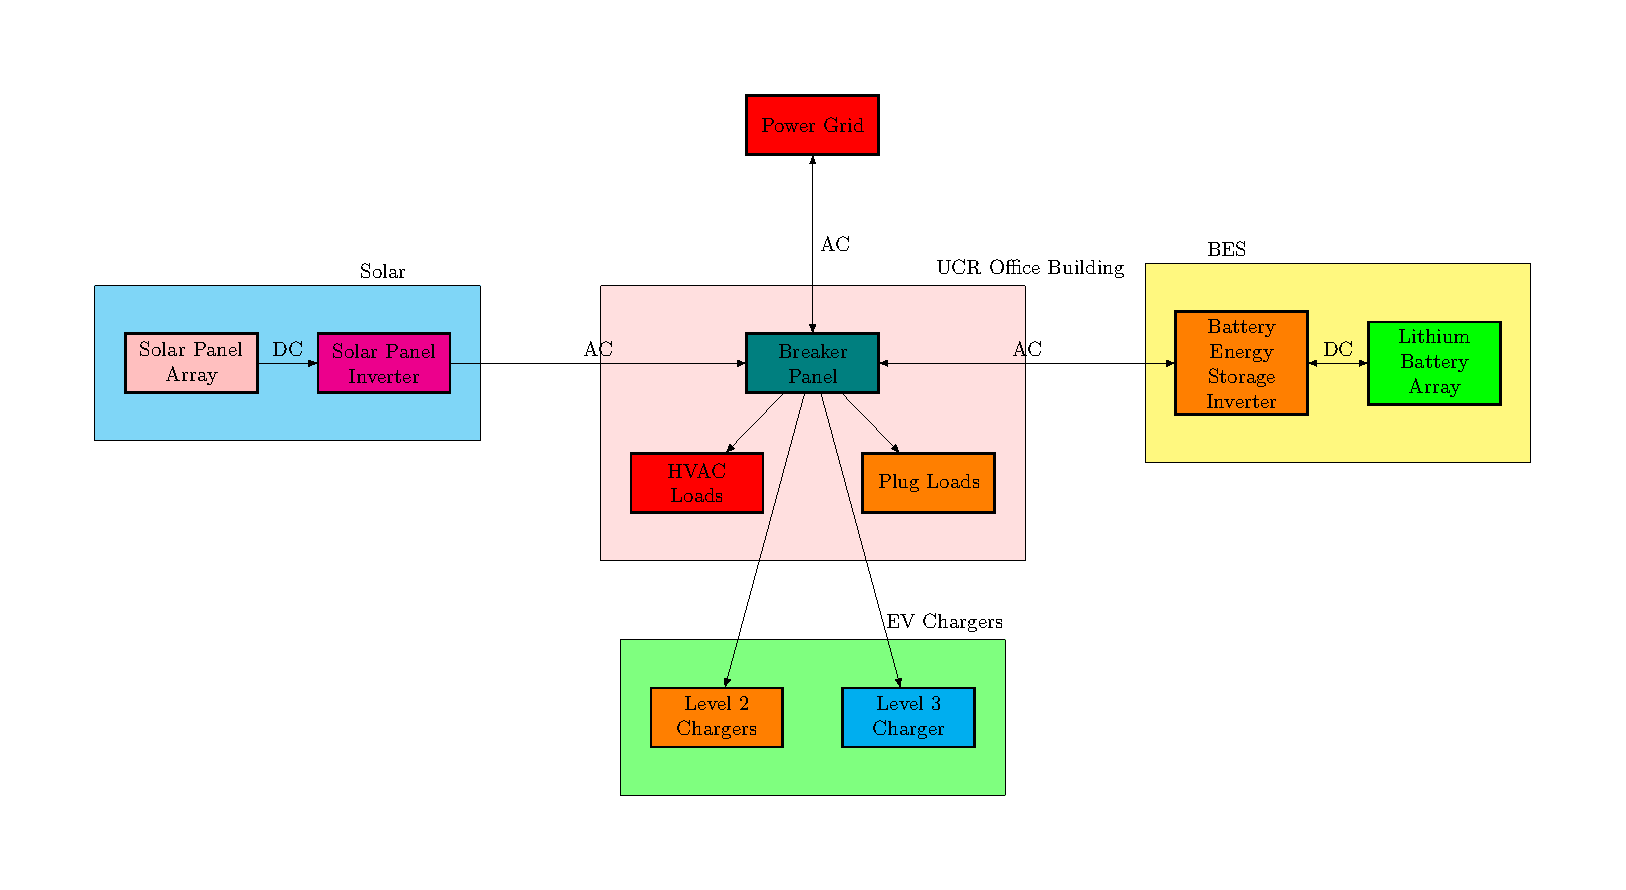
\includegraphics[width=1\linewidth]{Fig/power_system_setup_modelica}
		\caption{Microgrid Architecture}
		\label{fig:powersystemsetupfull}
	\end{figure}
	\subsection{Validation}
		To ensure that our model accurately portrays our real world system, a year of real world data was used to validate the $P_G $ output . $P_G$ is defined as the power the microgrid sends or consumes from the grid.  The actual data was compared to the simulated  with a correlation coefficient of  $\approx$ 0.965087 as shown in Figure \ref{fig:ucr15minutedatamar012022tomar012023}. 
		\begin{figure}[H]
			\centering
			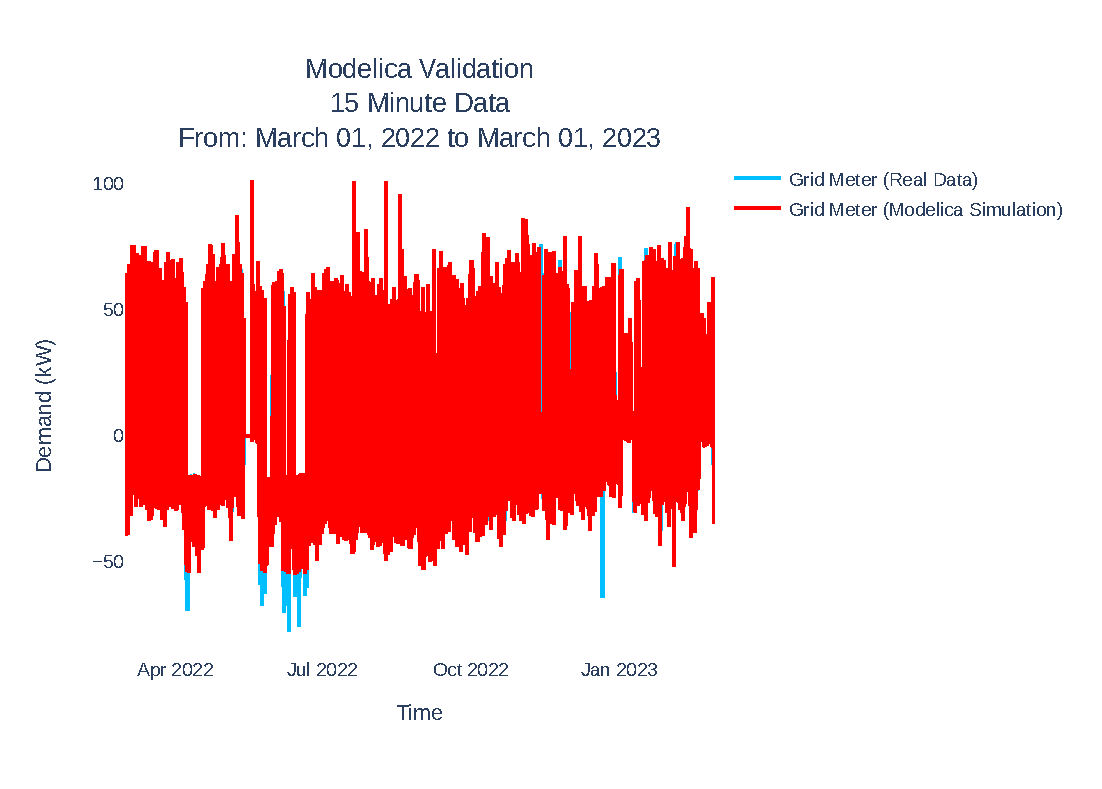
\includegraphics[width=1\linewidth]{Fig/ucr_15_Minute_Data_Mar_01_2022_to_Mar_01_2023}
			\caption{Whole Year Validation}
			\label{fig:ucr15minutedatamar012022tomar012023}
		\end{figure}
    \subsection{Solar Generation and Building Loads}
    	The solar power in our model is based on the historical solar data from our 100 kW  photovoltaic (PV) array. The HVAC loads and the regular building loads are represented separately in this model but utilize the same method; they both use historical real world power data to represent their load in the system. 
    \subsection{EV Charger Loads }
   		Our model also considers transportation loads in the form of EV chargers. The EV chargers are represented as two models: Level 2 EV chargers, and Level 3 EV chargers. While other building loads follow a typical daily and yearly pattern, EV loads are different since they stochastically switch on and off. Our case study microgrid has four Level 2 chargers, so it can have four ``steps'' of 7.2 kW each, while there is only one ``step'' of 50 kW with the Level 3 chargers. To generate EV loads in our model, we use a Poisson random distribution to generate the number of charge sessions in a day, the arrival times, and charging durations based on real world data recorded over a year. 
		\begin{figure}[H]
			\centering
			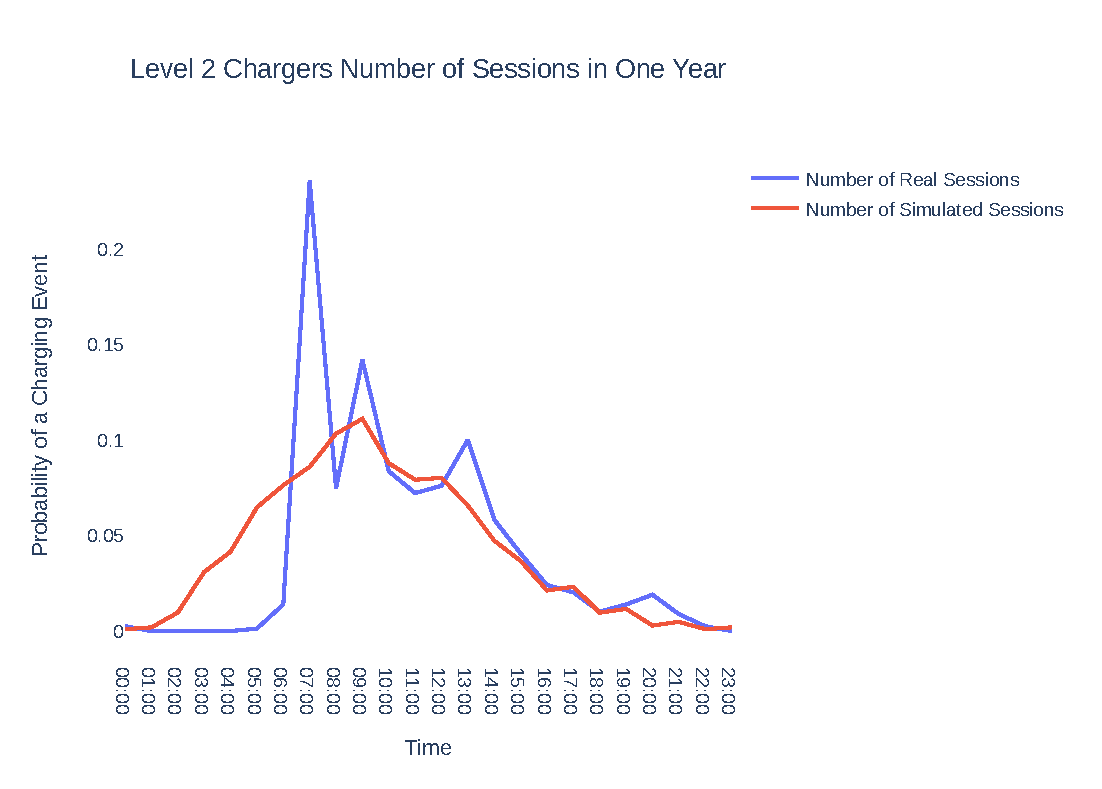
\includegraphics[width=1\linewidth]{Fig/l2_avg_day_rand_poisson_1_hour_pdf}
			\caption{Probability Density Function of the Level 2 EV Charger Validation}
			\label{fig:l2avgdayrandpoisson1hourpdf}
		\end{figure}
		\begin{figure}[H]
			\centering
			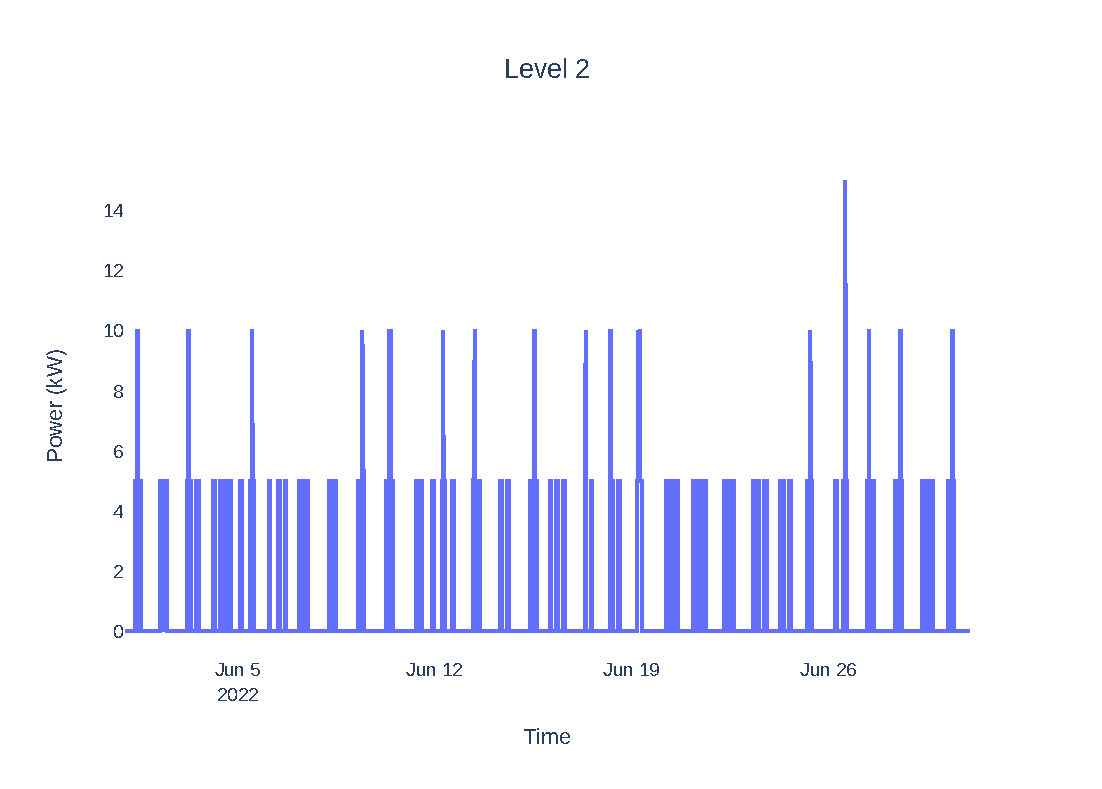
\includegraphics[width=1\linewidth]{Fig/l2_g_pad_poisson_June}
			\caption{Level 2 Chargers Simulated Power Draw}
			\label{fig:l2gpadpoissonjune}
		\end{figure}
%   		However, the number of sessions and duration is reduced to X and Y for the Level 3 charger.  
%		\begin{figure}[H]
%			\centering
%			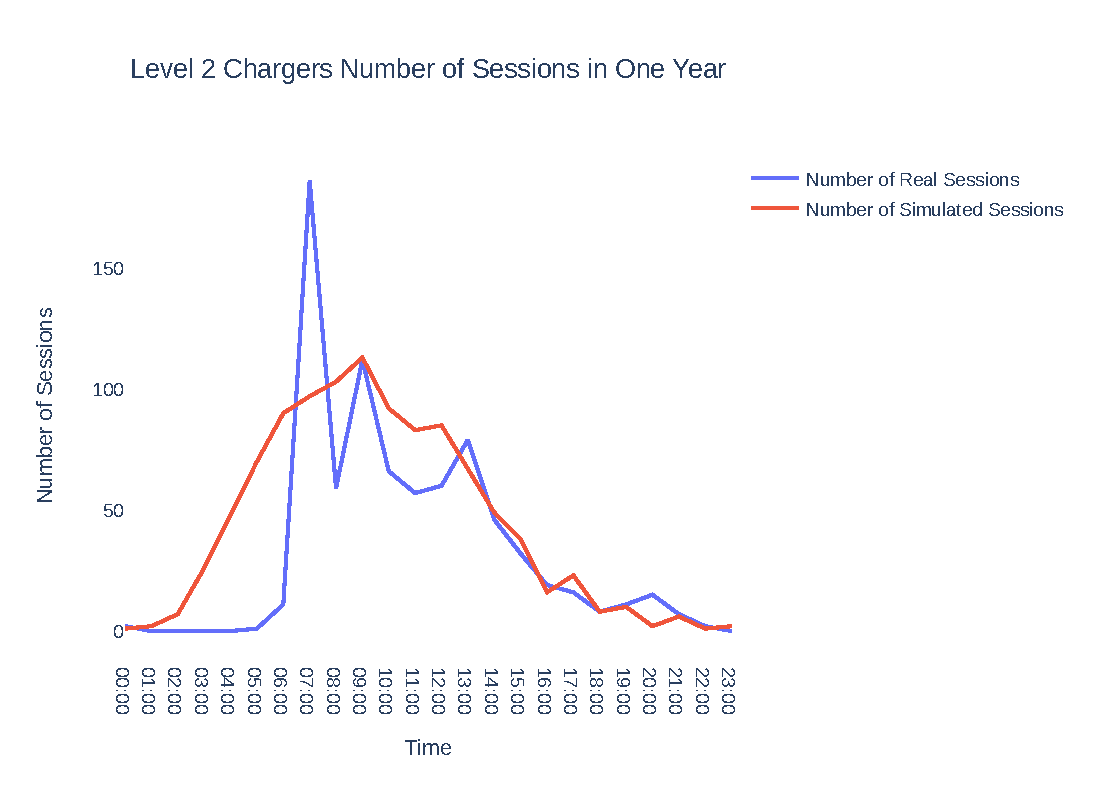
\includegraphics[width=1\linewidth]{Fig/l2_avg_day_rand_poisson_1_hour}
%			\caption{Number of Real and Simulated Sessions}
%			\label{fig:l2avgdayrandpoisson1hour}
%		\end{figure}
%		Historical data was collected from the Level-2 charger to determine the parameters for the Poisson random generator, following a typical daily charge pdf shown in Figure \ref{fig:l2avgdayrandpoisson1hourpdf}, and the power output of the Level 2 chargers in Figure \ref{fig:l2gpadpoissonjune}. After analyzing the historic data, three peak charging usually occur at $[7, 9, 13]$ with the average number of cars arriving during each peak being $[6, 2, 1]$. A mean charging time of 90 minutes is assumed. Using these two parameters, the EV random arrivals functions generates random arrivals times and duration. The function uses numpy, a Python library, to create a Poisson random distribution with the means centered around the peak times. The random data has a seed value of 10, so that every EV charging load event in the different scenarios is the same to prevent any higher demand event being solely attributed to an outlier event from the EV charging load. The random arrivals for Level 3 charging is modeled as have three peak time: $[7, 9, 13]$, number of vehicle arrivals: $[2, 1, 1]$, and a charging mean time of 30 minutes.  
	Historical data from the Level-2 charger was utilized to determine the parameters for the Poisson random generator, consistent with the typical daily charge probability density function (PDF) depicted in Figure \ref{fig:l2avgdayrandpoisson1hourpdf}. Additionally, the power output of the Level-2 chargers is illustrated in Figure \ref{fig:l2gpadpoissonjune}. Analysis of the historical data revealed three distinct peak charging periods occurring at $[7,9,13]$ hours, with average vehicle arrivals during each peak of $[6,2,1]$, respectively. A mean charging time of 90 minutes was assumed. Leveraging these parameters, the EV random arrivals function generates random arrival times and durations. The function employs the NumPy library in Python to create a Poisson random distribution with means centered around the peak times. To ensure consistency across different scenarios and prevent any outlier event from the EV charging load disproportionately influencing higher demand events, a random data seed value of 10 was employed to ensure every charging event is the same. The random arrivals for Level 3 charging are modeled with three peak times at $[7,9,13]$ hours, an average vehicle arrival count of $[2,1,1]$, and a mean charging time of 30 minutes.
		
			
%		\begin{figure}[H]
%			\centering
%			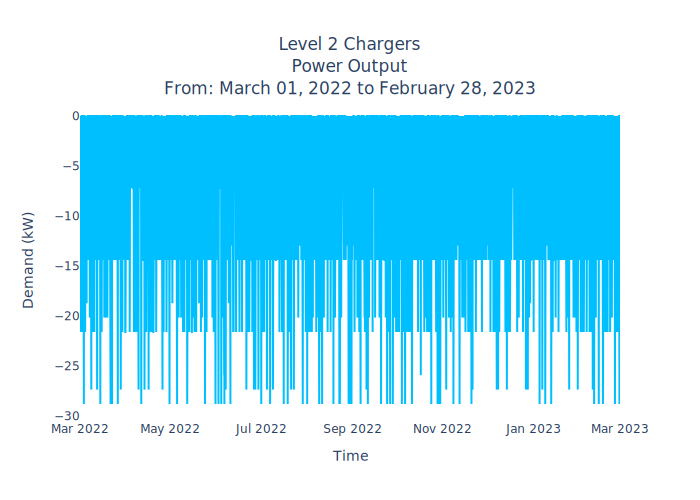
\includegraphics[width=1\linewidth]{Fig/ev_l2_po}
%			\caption{Level 2 Power Output}
%			\label{fig:evl2po}
%		\end{figure}
    
    \subsection{BESS and Peak Shaving}
    	The BESS is modeled as a battery connected to a bidirectional inverter. The BESS output is controlled by generated data from the control algorithm. The BESS output is computed in real-time by using a peak shaving algorithm utilizing  BESS SOC and the grid meter output. The algorithm charges the battery when excess solar power is exported to the grid, and when the battery needs to be charged. Python code reads the net load from the grid  model and determines the amount of CO\textsubscript{2} being produced during that interval.  Algorithm \ref{alg:peakshavingflatrate} shows the peak shaving algorithm sufficient for a flat rate demand response. 
%    	However,  for a TOU pricing structure, both energy and demand charges are assumed to be TOU rates with no additional flat rate demands. The TOU peak shaving algorithm is presented in Equation 1 with a simple objective to minimize the amount of power the microgrid pulls from the grid while accounting for energy and demand charges. The minimization objective is accomplished by optimizing for the summation of  TOU energy ($\Delta t \boldsymbol{\alpha}^{\boldsymbol{T}} \boldsymbol{P}^G$) and the maximums TOU demands ($\max \left(\boldsymbol{\beta}^{\text {On }} \boldsymbol{P}^G\right)+\max \left(\boldsymbol{\beta}^{\text {Mid }} \boldsymbol{P}^G\right)+\max \left(\boldsymbol{\beta}^{\text {Off }} \boldsymbol{P}^G\right)$). This algorithm is further described and validated in \cite{hasan2023universal},  \cite{hasan2021comprehensive} . \\
%%		\begin{figure}
%%			\centering
%%			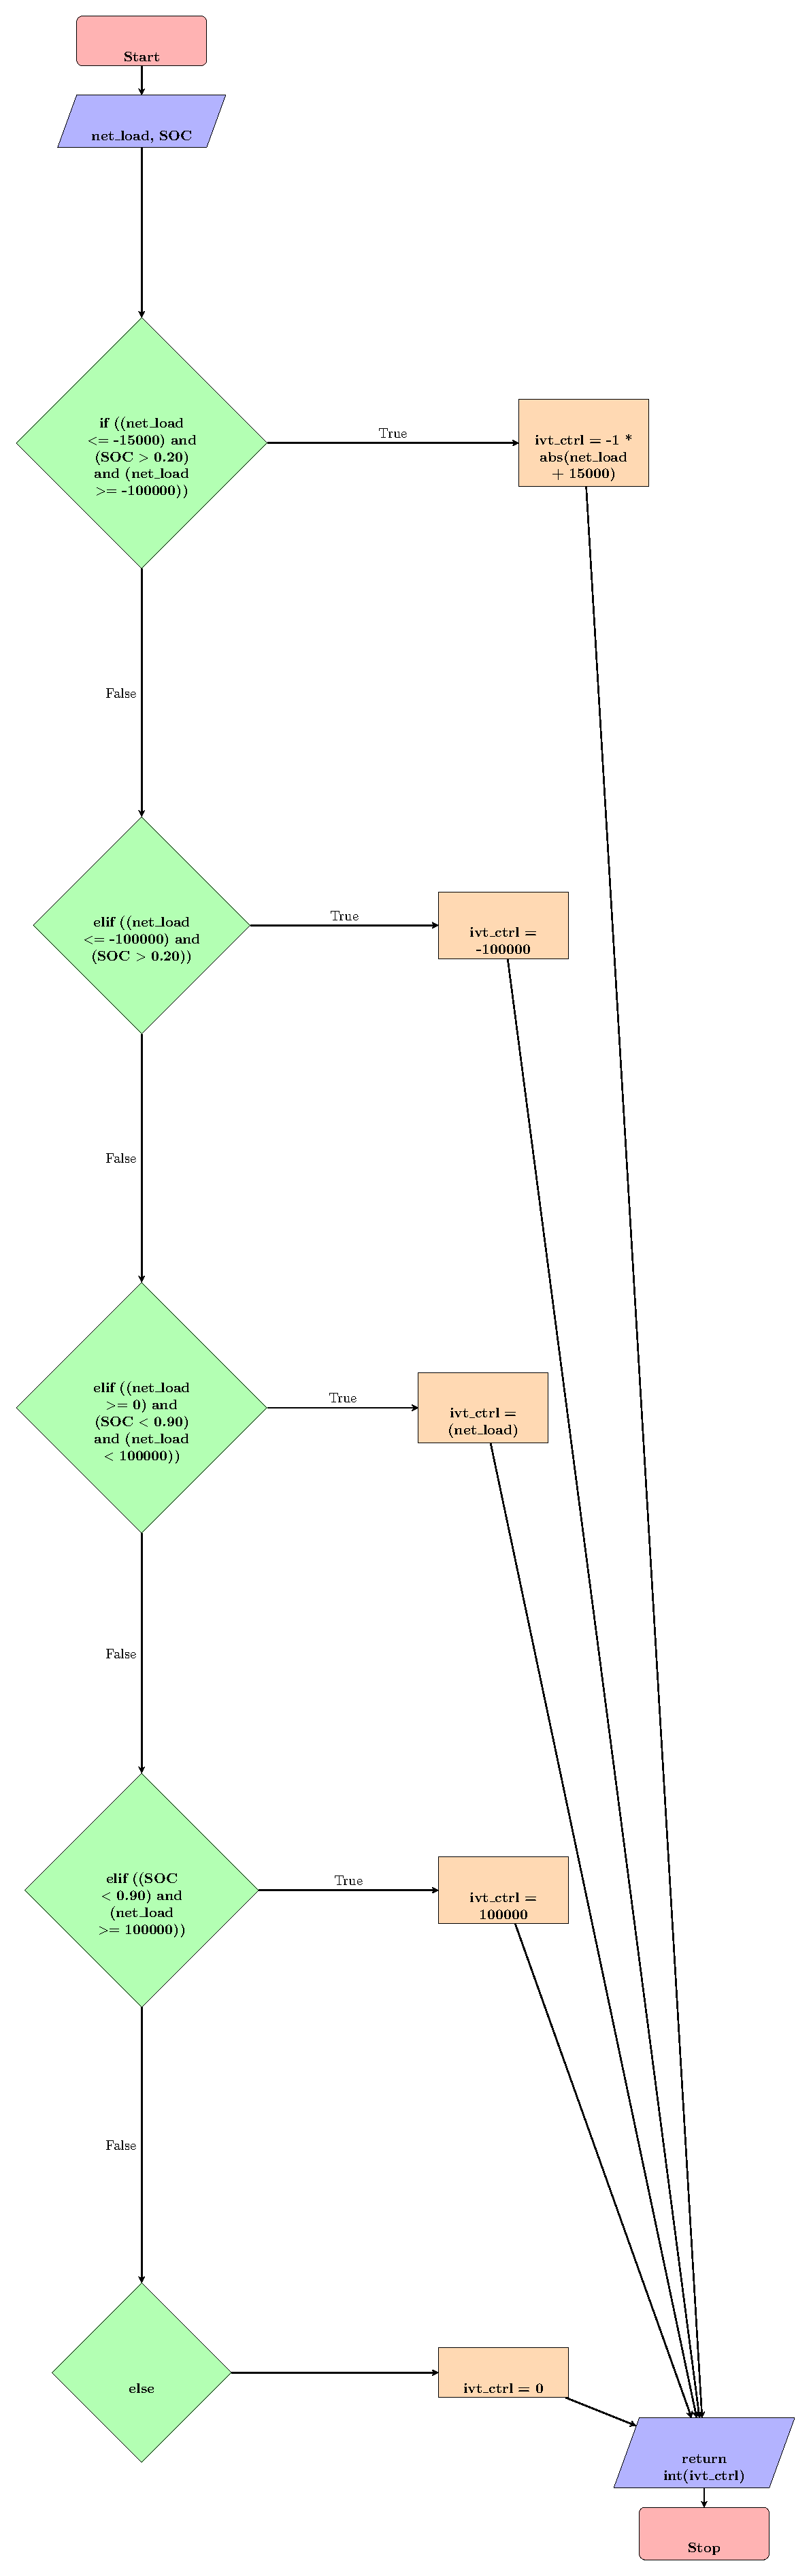
\includegraphics[width=0.7\linewidth]{Fig/peak_shaving_flat_rate}
%%			\caption{Flat Rate Peak Shaving Algorithm Flowchart}
%%			\label{fig:peakshavingflatrate}
%%		\end{figure}
%			\normalsize
%			\footnotesize
%		\begin{equation} 
%			\min f\left(\boldsymbol{P}^G\right)=\Delta t \boldsymbol{\alpha}^{\boldsymbol{T}} \boldsymbol{P}^G+\max \left(\boldsymbol{\beta}^{\text {On }} \boldsymbol{P}^G\right)+\max \left(\boldsymbol{\beta}^{\text {Mid }} \boldsymbol{P}^G\right)+\max \left(\boldsymbol{\beta}^{\text {Off }} \boldsymbol{P}^G\right)
%		\end{equation}
%		\normalsize
%		subject to
%		$$
%		\begin{aligned}
%			& E_{t+1}^B=E_t^B+P_t^B \cdot \Delta t, \forall t \in \boldsymbol{T}^{\mathbf{t o t}} \\
%			& E^{B m i n} \leq E_t^B \leq E^{B m a x}, \forall t \in \boldsymbol{T}^{\mathbf{t o t}} \\
%			& P_t^B=P_t^{B+}-P_t^{B-}, \forall t \in \boldsymbol{T}^{\text {tot }} \\
%			& 0 \leq P_t^{B+} \leq \delta_t P^{B+\max }, \forall t \in \boldsymbol{T}^{\mathbf{t o t}} \\
%			& 0 \leq P_t^{B-} \leq\left(1-\delta_t\right) P^{B-\max }, \forall t \in \boldsymbol{T}^{\mathbf{t o t}} \\
%			& 0 \leq \delta_t \leq 1, \forall t \in \boldsymbol{T}^{\mathbf{t o t}} \\
%			& P_t^{B+}=\eta^{+} P_t^{S B}, \forall t \in \boldsymbol{T}^{\mathbf{t o t}} \\
%			& P_t^S=P_t^{S B}+P_t^{S L}, \forall t \in \boldsymbol{T}^{t o t} \\
%			& P_t^L=P_t^{S L}+P_t^{B L}+P_t^G, \forall t \in \boldsymbol{T}^{\text {tot }} \\
%			& P_t^{B L}=\eta^{-} P_t^{B-}, \forall t \in \boldsymbol{T}^{t o t} \\
%			& P_t^{S L} \geq 0, \forall t \in \boldsymbol{T}^{t o t}
%		\end{aligned}
%		$$

		\begin{algorithm}
			net\_load, SOC $\gets$ Modelica Data Output
			\uIf{if condition}{net\_load  <=   -15 kW and SOC > 20 \%  and net\_load  >=  -100 kW
				BESS\_inverter = -net\_load  - 15 kW
			}
			\uElseIf{net\_load  <= -100 kW and SOC > 20 \%}{
					BESS\_inverter = -100 kW
			}
			\uElseIf{net\_load  >=  0 kW and SOC < 90 \%  and net\_load  <=  100 kW}{ 
				 BESS\_inverter = -net\_load
			}
			\uElseIf{net\_load  >=  0 kW and SOC < 90 \%  }{
				 BESS\_inverter = 100 kW
			}
			\Else{
				BESS\_inverter = 0
			}
			\caption{Peak Shaving}
			\label{alg:peakshavingflatrate}
		\end{algorithm}

\section{Results}
		The charging setup is modified in OpenModelica for different layouts and scenarios. The scenarios are described in Table \ref{tab:scenarios}.\\
		Scenario 1 represents the baseline case where only the building loads, such as the air conditioners, appliances, and lights, are connected to the grid. Scenario 2 represents the case where a building installs four Level 2 and one Level 3 charger. Scenario 3 is the first case that utilizes a microgrid, which includes 100 kW of solar power and 500 kWh of battery storage. This scenario demonstrates the peak-shaving capabilities of a microgrid without EV chargers, creating a high demand. This can be thought of as the baseline case for the BESS microgrid. Scenarios 4, 5, 6, 7, and 8 represent a transportation microgrid with EV chargers; the BESS capacity is varied to different sizes to show which BESS size offers the lowest cost and the lowest CO\textsubscript{2} emissions. \\
		Each scenario is run independently of the other, and the power outputs of the different components in the simulation are shown in Figure \ref{fig:scenariospoweroutputboxplot}. Scenarios 1 and 2 are constantly negative, meaning they pull power from the grid. Scenarios 3-8, on the other hand, are mostly positive or limited to -15 kW, meaning it either exports power to the grid or consumes only 15 kW. The reason for the 15-kW floor is that with the utility company's electric rate, a minimum of 15 kW is charged for the demand, meaning that a zero-demand microgrid will not make a financial difference for the user. \\
		While the peak shaving algorithm should limit the amount of power consumed at any time to 15 kW, there are still times when the BESS cannot supply the building with power. This happens when the BESS is too depleted, and there is little to no solar power to replenish it, as shown in Figure \ref{fig:scenario3peakshaving}. The two main reasons for these events are multiple cloudy days and electrical faults. The larger the battery capacity, the depletion of the battery occurs less frequently, and the microgrid can better weather events of low solar output. During the winter months, most of the low solar power events occur. \\
		Figures \ref{fig:scenariospoweroutputboxplot}, \ref{fig:0scnoutputrun2mar012022tomar312022}, and \ref{fig:4scnoutputrun2jul012022tojul312022} show box plots of the power output. Figure \ref{fig:scenariospoweroutputboxplot} is for the entire year, while Figures \ref{fig:0scnoutputrun2mar012022tomar312022} and \ref{fig:4scnoutputrun2jul012022tojul312022} show selected months. The box plots show that all three figures' mean and 75th percentile are almost identical at 15 kW. This implies that peak shaving is functioning correctly most of the time. However, the outliers show when the BESS fails to keep the power pulled from the grid at 15 kW. \\	
		Just one outlier will change the demand charge for the entire billing month. In some months, the maximum demand peak of Scenario 2 and 3 are similar since they have the same load, but for most of the months, it is reduced significantly, reflected in the reduced demand charges of the building. Figure \ref{fig:netloadscenariocomparisonsummer} juxtaposes each scenario's power pulled from the grid. \\
		The average daily CO\textsubscript{2} emissions from each scenario are shown in Figure \ref{fig:emissionsscenariocomparison}. Scenario 2, with its increased charging events, shows about a 26\% increase of CO\textsubscript{2} emissions compared to Scenario 1. The CO\textsubscript{2} emissions from the transportation microgrids are lower than a conventional building, even with the additional load from the EV chargers. While adding 17\% to 45\% more CO\textsubscript{2} emissions compared to a microgrid without EV charging infrastructure (Scenario 3), those CO\textsubscript{2} emissions are easily offset by charging an average of 12 EVs per day. Table \ref{tab:emissions} shows each scenario's emissions and electric price amounts.
	\begin{table}[H]
		\caption{Simulated Scenarios of the UCR Microgrid using Different Layouts and Electric Pricing Structures}
		\tiny
		\begin{tabularx}{\linewidth}{l | l}
\toprule
 Scenario &  \\
\midrule
		1  & Standard Building with no EV Chargers\\
        2 & Standard Building with Level 2 and Level 3 Charging\\
        3 & Microgrid Building with 100 kW Solar, 500 kWh BESS, No EV Charging \\
        4 & Microgrid Building with 100 kW Solar, 100 kWh BESS, Level 2, and Level 3 Charging\\
        5 & Microgrid Building with 100 kW Solar, 250 kWh BESS, Level 2, and Level 3 Charging\\
        6 & Microgrid Building with 100 kW Solar, 500 kWh BESS, Level 2, and Level 3 Charging\\
        7 & Microgrid Building with 100 kW Solar, 1 MWh BESS, Level 2, and Level 3 Charging\\
        8 & Microgrid Building with 100 kW Solar, 1 MWh BESS, Level 2, and Level 3 Charging\\
\bottomrule
\end{tabularx}

		\normalsize
		\label{tab:scenarios}
	\end{table}
	
	\begin{figure}[H]
		\centering
		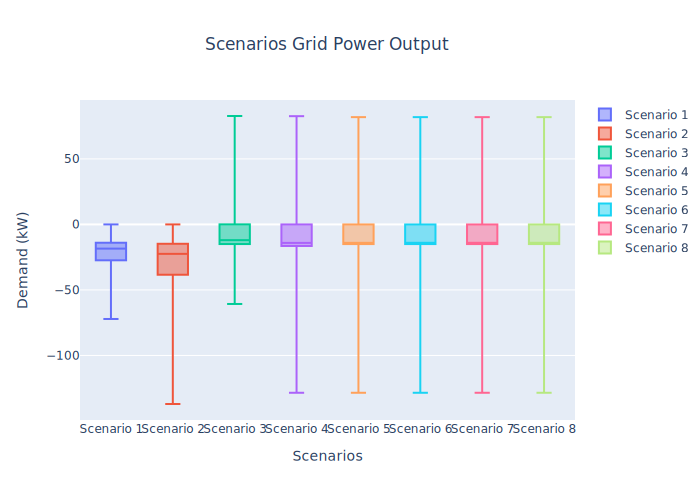
\includegraphics[width=0.9\linewidth]{Fig/scenarios_power_output_boxplot}
		\caption{Power measured from the meter}
		\label{fig:scenariospoweroutputboxplot}
	\end{figure}
	
	\begin{figure}[H]
		\centering
		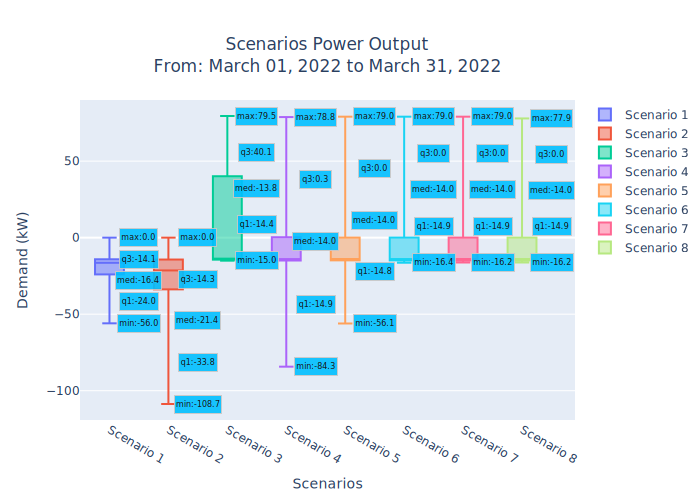
\includegraphics[width=1\linewidth]{Fig/0_Scn_Output_Run_3_Mar_01_2022_to_Mar_31_2022}
		\caption{Power measured from the meter for the month of March}
		\label{fig:0scnoutputrun2mar012022tomar312022}
	\end{figure}

	\begin{figure}[H]
		\centering
		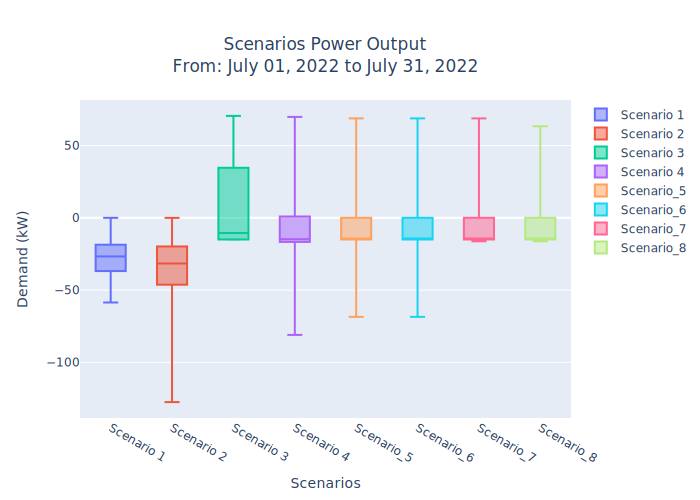
\includegraphics[width=1\linewidth]{Fig/4_Scn_Output_Run_3_Jul_01_2022_to_Jul_31_2022}
		\caption{Power measured from the meter for the month of July}
		\label{fig:4scnoutputrun2jul012022tojul312022}
	\end{figure}
	
%	\begin{figure}[H]
%		\centering
%		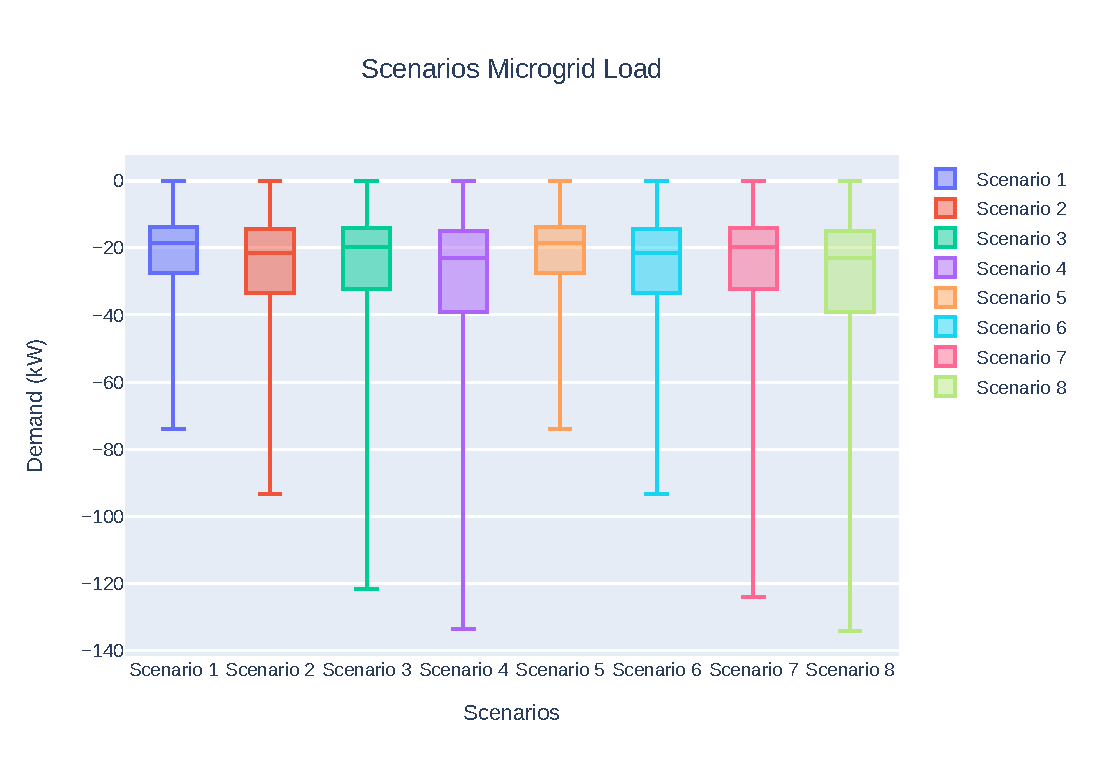
\includegraphics[width=0.9\linewidth]{Fig/scenarios_mg_load_output_boxplot}
%		\caption{Load of all the microgrid components}
%		\label{fig:scenariosmgloadoutputboxplot}
%	\end{figure}
	



    
	\begin{figure}[H]
		\centering
		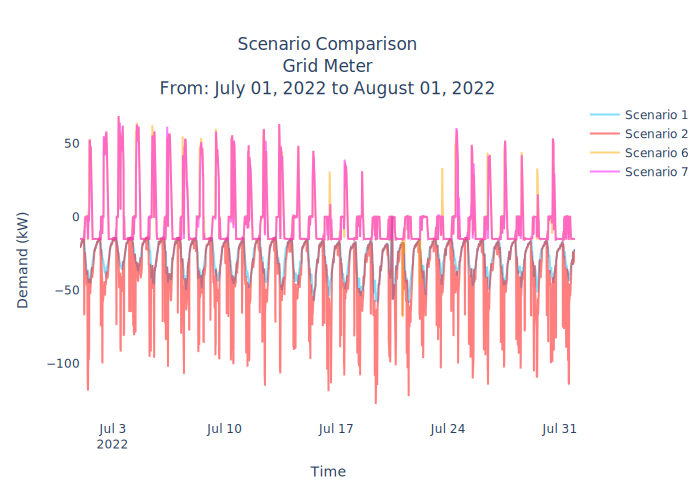
\includegraphics[width=1\linewidth]{Fig/net_load_scenario_comparison_summer_run_3}
		\caption{Summer Net Load Scenario Comparison}
		\label{fig:netloadscenariocomparisonsummer}
	\end{figure}
	
	
	\begin{figure}[H]
		\centering
		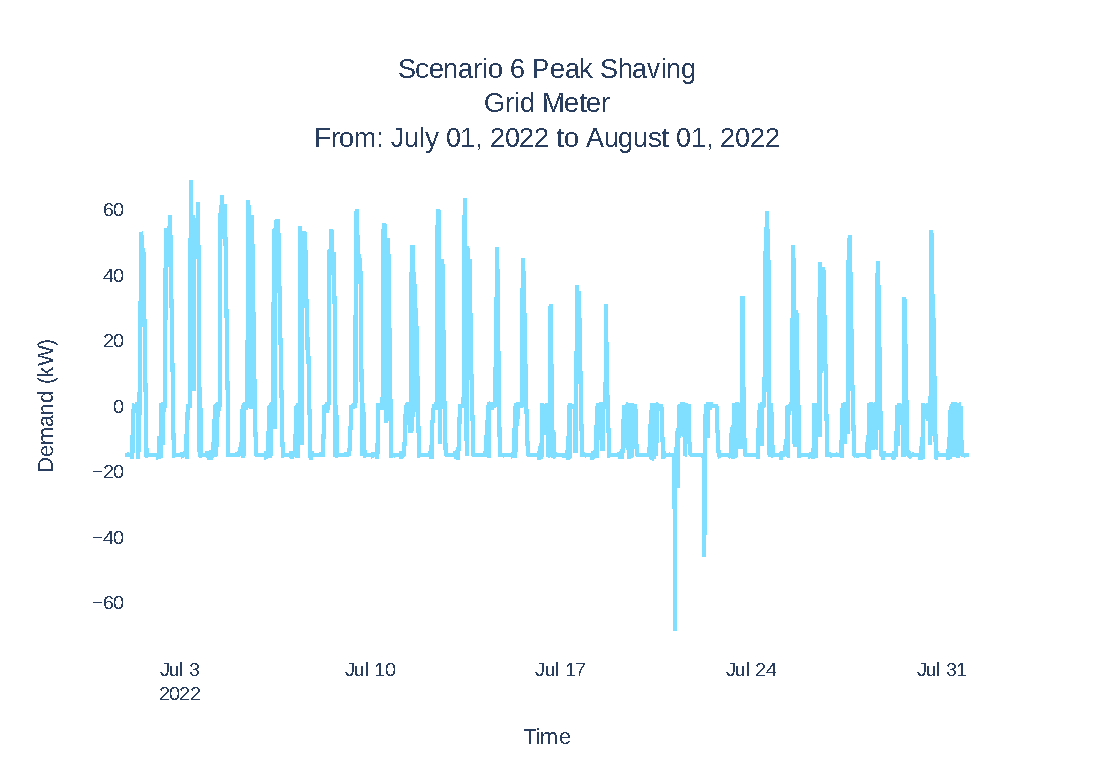
\includegraphics[width=1\linewidth]{Fig/scenario_6_peak_shaving}
		\caption{Peak Shaving Failure after Battery Depletion (500 kWh)}
		\label{fig:scenario3peakshaving}
	\end{figure}
	
	\begin{figure}[H]
		\centering
		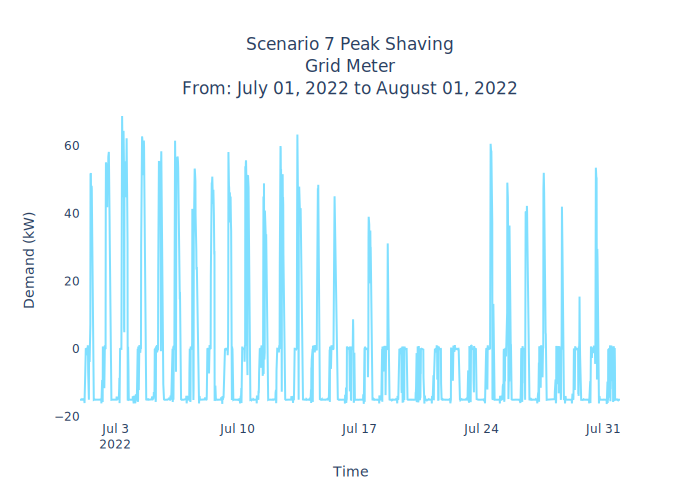
\includegraphics[width=1\linewidth]{Fig/scenario_7_peak_shaving}
		\caption{Peak Shaving Success with 1 MWh battery}
		\label{fig:scenario4peakshaving}
	\end{figure}

	\begin{figure}[H]
		\centering
		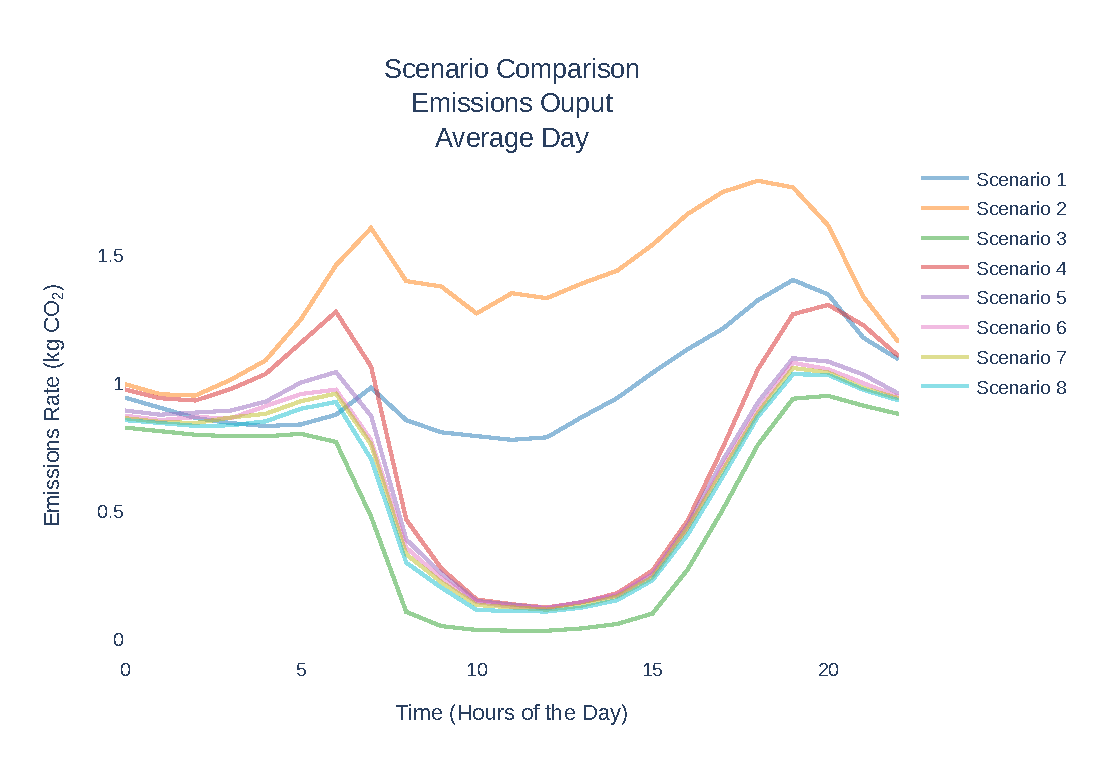
\includegraphics[width=1\linewidth]{Fig/emissions_scenario_comparison_run_3}
		\caption{CO\textsubscript{2} Emissions Outputs Averages During Times of Day, using a microgrid setup}
		\label{fig:emissionsscenariocomparison}
	\end{figure}
	
	\begin{table}[H]
		\caption{Microgrid Utility Prices and CO\textsubscript{2} Emissions Output under Different Pricing Scenarios and Pricing Structures}
		\tiny
		\centering
		\input{Table/kw_kwh_CO2_run_4.tex}
		\normalsize
		\label{tab:emissions}
	\end{table}	
		
	\begin{figure}[H]
		\centering
		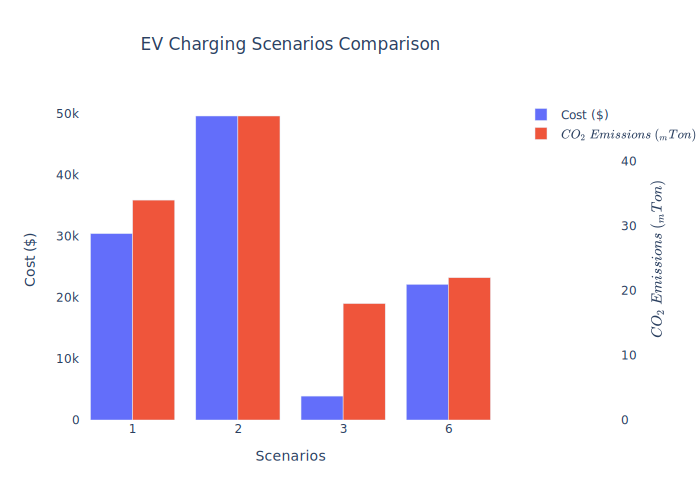
\includegraphics[width=1\linewidth]{Fig/mg_scene_comparison}
		\caption{EV Charging Scenarios Comparison}
		\label{fig:mgscenecomparison}
	\end{figure}
	
	\begin{figure}[H]
		\centering
		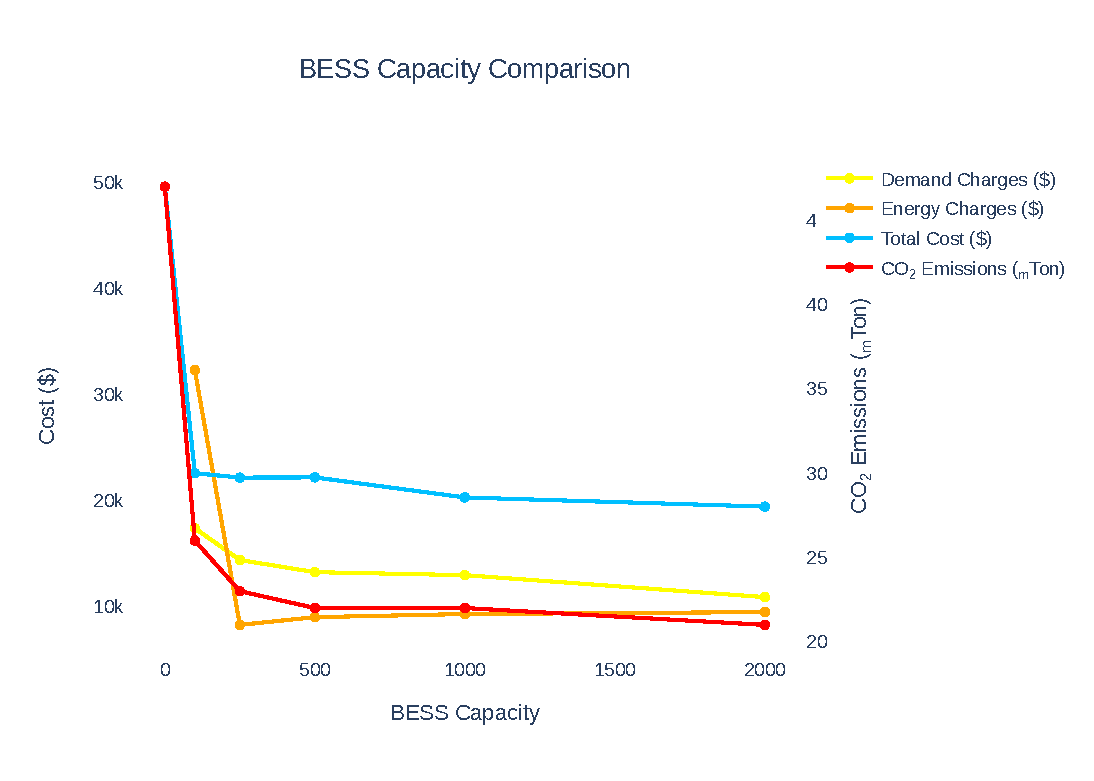
\includegraphics[width=1\linewidth]{Fig/bess_capacity_comparison}
		\caption{Cost and CO\textsubscript{2} Emissions for Different Battery Capacities}
		\label{fig:besscapacitycomparison}
	\end{figure}

	\section{Conclusions}
		Transportation microgrids have emerged as a compelling solution for mitigating the electrical costs and emission levels associated with EV charging infrastructure. A comprehensive analysis of various scenarios reveals transportation microgrids' significant economic and environmental benefits compared to conventional systems, as depicted in Figure \ref{fig:mgscenecomparison}. For the transportation microgrid systems, the estimated annual savings range from \$8,000 to \$10,000, even with the additional demand from EV chargers. Compared to a building with EV chargers but without a microgrid, the annual savings are even more substantial, reaching \$27,000 to \$29,000. This implies that transportation microgrids can amplify the savings from switching from a conventional building by a factor of three. Furthermore, transportation microgrids can reduce CO\textsubscript{2} emissions by 24\% to 38\% compared to a conventional building and by 45\% to 55\% compared to a scenario where the building also has EV chargers. Consequently, users are strongly incentivized to adopt transportation microgrids rather than simply installing EV chargers at their buildings. \\
		
		It is important to note that, increasing the battery capacity does not necessarily guarantee improved microgrid performance. Figure \ref{fig:besscapacitycomparison} illustrates the different battery capacities evaluated in this microgrid setup. The largest capacity is 20 times the smallest battery, but the corresponding cost and CO\textsubscript{2} reductions are not 20-fold. Addressing the most challenging solar power outages requires a significant increase in battery capacity, while providing only marginal CO\textsubscript{2} and cost savings in return. As shown in the billing month of July in Figures \ref{fig:scenario3peakshaving} and \ref{fig:scenario4peakshaving}, doubling the battery capacity can eliminate some peaks from a couple of cloudy days. However, the additional savings of \$2,000 per year do not justify the cost of the extra capacity. Lastly, a 15 kW demand price floor has an adverse impact on CO\textsubscript{2} emissions, as it discourages users from maintaining a zero net load in a peak shaving setup. \\
		
		In conclusion, transportation microgrids represent a promising solution for reducing the environmental and economic impact of EV charging infrastructure. However, careful consideration of battery capacity and demand price structures is crucial to optimize the microgrid's performance and cost-effectiveness.

	\section{Future Work}
		  Future research will explore different, more advanced control strategies to optimize the electric costs and CO\textsubscript{2} emissions of the transportation microgrid. These strategies will include preventing users from charging during high peak times, maximizing the use of the clean energy produced by the solar panels, and minimizing the power drawn from the grid during high CO\textsubscript{2} times. The effect of the new net energy metering policy in California on the value of the BESS system will also be assessed.
%		\nocite{*}
		\bibliographystyle{IEEEtran}
		\bibliography{cite}
		
\end{document}
